% !TeX root = ../main.tex

\chapter{行人追踪算法}
  行人追踪算法blabla

  
\section{视觉行人追踪}
  计算机视觉中的行人追踪,主要包括密集跟踪方法,即基于行人检测和识别的追踪,以及稀疏跟踪方法,即基于目标动态的追踪。

  在密集跟踪方法中,我们实际上并没有“跟踪”物体,而是在视频不同的时间点的一系列帧上扫描和检测物体的位置。由于每次的目标检测都是独立地在当前帧上进行的,所以每次检测时,都需要处理图像中的所有像素,所以以这种方法进行目标跟踪,计算量会比较大。

  稀疏跟踪方法是根据物体的动态信息,对其可能的运动轨迹进行预测,并结合其上一帧所在位置和对当前帧的观察,得出其当前位置的算法。由于已知物体在上一帧时的位置,所以对当前帧识别时,只需要检测上一帧物体所在位置附近的像素,这样一来,相对于密集跟踪方法,就减少了大量的计算。此外,由于我们结合了对物体运动的预测和观察来进行估计,在一些情况下准确度也会较高,但在物体速度较快时,可能会失去对物体的追踪,当目标物暂时从视野中消失时,可能难以重新找回物体。

\subsection{基于检测的追踪}
  基于机器学习的方法是现阶段行人检测算法的主流,下面将介绍常用行人检测方法原理。

\subsubsection{人工特征+分类器}
\paragraph{常用特征描述子}

  特征描述子是一种对图片的表示方法,它通过提取图片中的关键信息并丢弃多余信息来对图片信息进行简化。通常地,特征描述子将一个RGB三通道的图片转化成一个特征向量。
  
  为了做到精确地进行图像识别、目标检测,我们必须首先明确什么是关键的、有用的信息,什么是冗余信息。

  a. 颜色直方图

  颜色特征具有旋转不变性,且不受目标的大小和形状的变化影响,在颜色空间中分布大致相同,从而具有较高的鲁棒性。

  颜色直方图是描述颜色特征最常用的描述子,它是是对目标表面颜色分布的统计,描述了不同色彩在图像中所占的比例,但无法描述图像中颜色的局部分布及每种色彩所处的空间位置,即无法描述图像中的某一具体的对象或物体。颜色直方图具有稳定性好、抗部分遮挡、计算方法简单和计算量小的特点。

  颜色直方图可以基于不同的的颜色空间,其中,最常用的是RGB空间和HSV空间。以RGB空间为例,分别统计每个像素的R、G、B数值落在[0,255]上每个点的频度,绘制出直方图,该图片的颜色特征即为三个长为256的向量,分别表示其的红色、绿色、蓝色的统计分布。以一张人物照片\ref{fig:ewan}为例,图\ref{fig:rgbhistogram}为其RGB颜色直方图。

\begin{figure}[htb]
  \centering
  
\includegraphics[width=0.3\textwidth]{ewan.jpg}
  \caption{原图}
  \label{fig:ewan}
\end{figure}

\begin{figure}[htb]
  \centering
  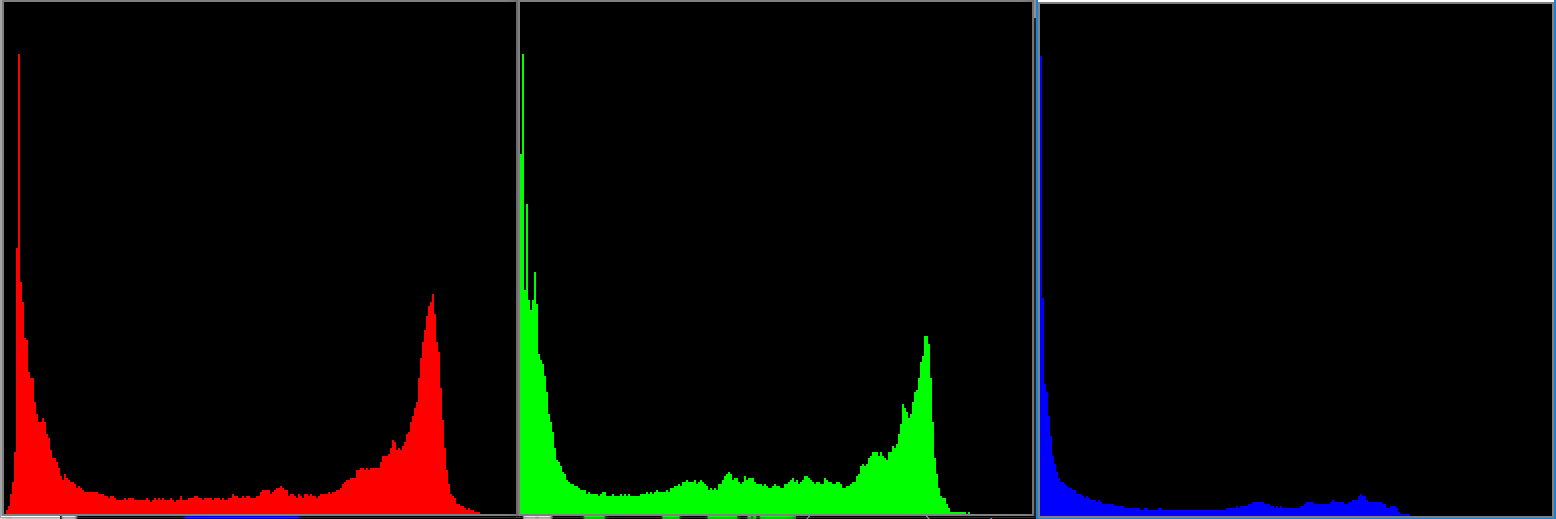
\includegraphics[width=0.7\textwidth]{rgb_histogram.png}
  \caption{左:B通道颜色直方图;中:G通道颜色直方图;右:R通道颜色直方图}
  \label{fig:rgbhistogram}
\end{figure}

  但RGB颜色空间的均匀性非常差,且两种颜色之间的直觉差异色差不能表示为改颜色空间中两点间的距离,RGB这三种颜色的分量的取值与所生成的颜色之间的联系并不直观。

  在计算机视觉中,我们常采用HSV颜色空间来表示颜色。HSV是一种将RGB色彩空间中的点在圆柱坐标系中的表示方法,相对于RGB,它能够更加直观地表示色彩的明暗、色调以及鲜艳程度,方便进行颜色之间的对比。此外,由于HSV单独提取了颜色的明暗,也可以一定程度上抵抗光照明暗带来的影响。\citet{sural2002segmentation}的实验显示,使用HSV直方图进行行人识别的结果相比RGB直方图有了明显提高。

  HSV即色相(Hue)、饱和度(Saturation)、亮度(Value)。色相即表示物体的颜色,如红色、黄色等,在$0^{\circ}$到$360^{\circ}$的标准色轮上,按位置度量色相;饱和度是指颜色的强度或纯度,表示色相中灰色分量所占的比例,它使用从0\%(灰色)至100\%(完全饱和)的百分比来度量;亮度是颜色的相对明暗程度,通常使用从0\%(黑色)至100\%(白色)的百分比来衡量。

\begin{figure}[htb]
  \centering
  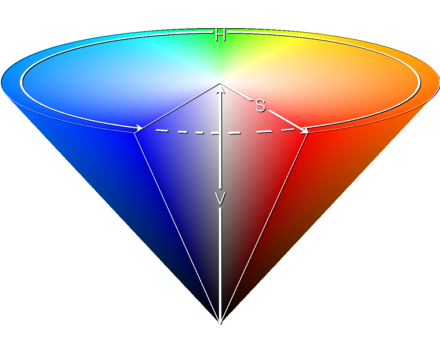
\includegraphics[width=0.4\textwidth]{hsv.png}
  \caption{HSV模型可以使用圆柱坐标系中的一个圆锥形子集表示}
  \label{fig:hsv}
\end{figure}

  由于大部分数字图像都是基于RGB空间进行表示的,我们需要首先把RGB空间坐标映射到HSV空间。给定$(r,g,b)$分别是一个颜色的红、绿、蓝坐标,它们的值是在0到1之间的实数,$max$为$r$,$g$和$b$之中的最大值,$min$为其中的最小值,则从$(r,g,b)$到$(h,s,v)$的转换公式如下:\cite{foley1982fundamentals}

$$h={\begin{cases}0^{\circ }&{\mbox{if }}max=min\\60^{\circ }\times {\frac  {g-b}{max-min}}+0^{\circ },&{\mbox{if }}max=r{\mbox{ and }}g\geq b\\60^{\circ }\times {\frac  {g-b}{max-min}}+360^{\circ },&{\mbox{if }}max=r{\mbox{ and }}g<b\\60^{\circ }\times {\frac  {b-r}{max-min}}+120^{\circ },&{\mbox{if }}max=g\\60^{\circ }\times {\frac  {r-g}{max-min}}+240^{\circ },&{\mbox{if }}max=b\end{cases}}$$

$$s={\begin{cases}0,&{\mbox{if }}max=0\\{\frac  {max-min}{max}}=1-{\frac  {min}{max}},&{\mbox{otherwise}}\end{cases}}$$

$$
v=max
$$

  HSV直方图的计算与RGB类似,只是将颜色空间有所差异,我们同样使用图片\ref{fig:ewan}计算其HSV直方图,见图\ref{fig:hsvhistogram}。

\begin{figure}[htb]
  \centering
  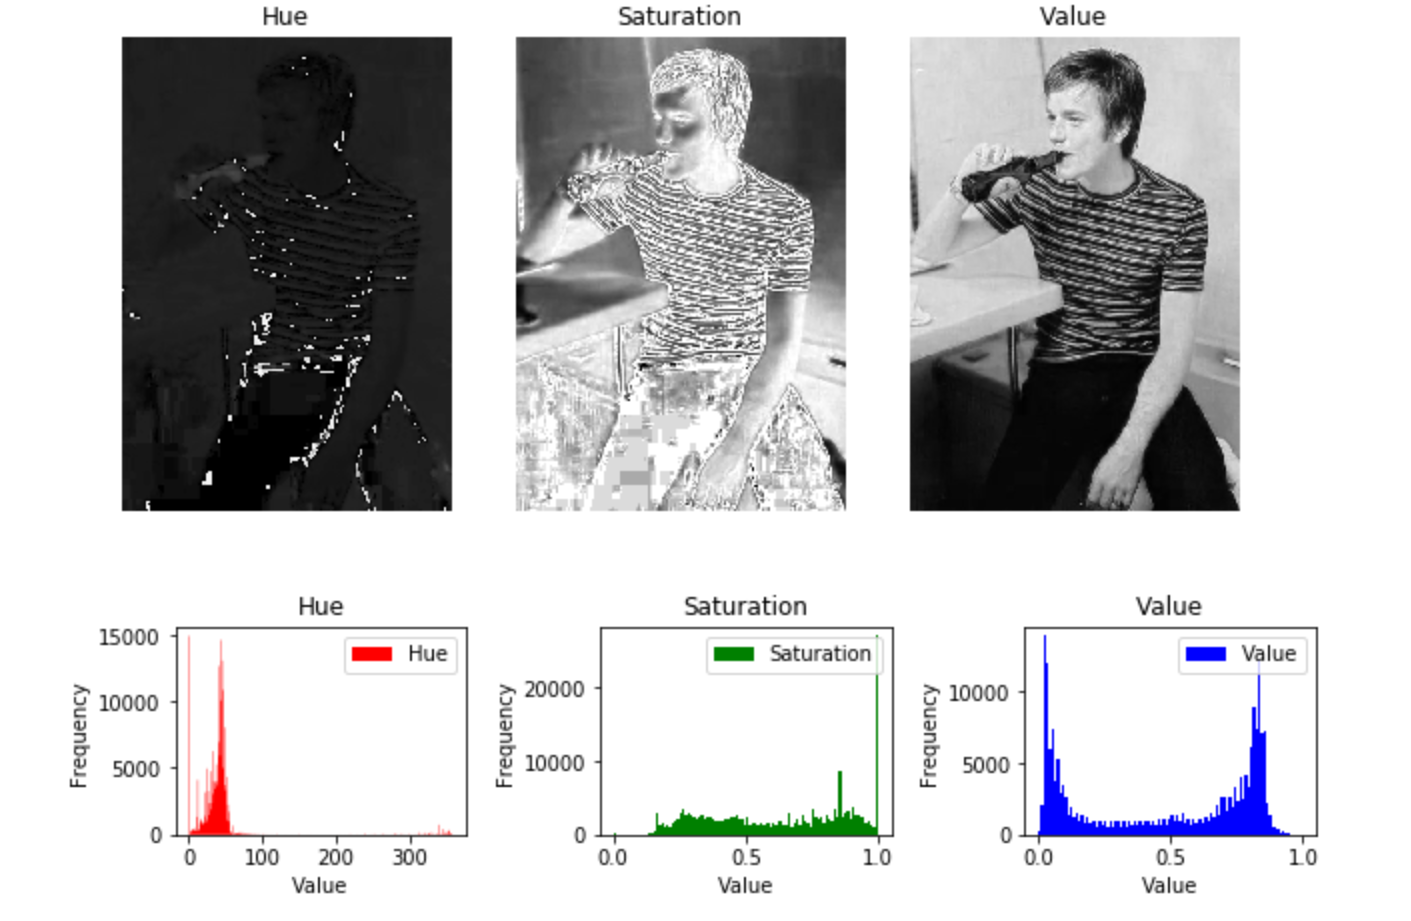
\includegraphics[width=1.0\textwidth]{hsv_histogram.png}
  \caption{左:H通道灰度图和颜色直方图;中:S通道灰度图和颜色直方图;右:V通道灰度图和颜色直方图}
  \label{fig:hsvhistogram}
\end{figure}

  b. 方向梯度直方图

  方向梯度直方图(Histogram of Oriented Gradient, HOG)是目前行人识别中最广泛使用的特征描述子之一。\citet{dalal2005histograms}在2005年提出HOG结合SVM(支持向量机,support vector machine)进行行人检测的方法,在此之后,该方法被广泛应用到了图像识别中,并尤其在行人检测中获得了巨大的成功,也出现了很多改进和变体。

  在HOG特征描述符中,它通过计算和统计图像局部区域的梯度方向直方图来构成特征。由于在物体的边缘和角落处图片的颜色会进行突变,故在这些区域,梯度的大小会很大,显然,边缘和角落比起平坦区域包含更多关于物体形状的信息。而通过对边缘和角度的描述,HOG正可以很好地描述局部目标的表面质地和形状信息。

  为了计算方向梯度,我们可以简单地使用内核(Kernel)$[-1,0,1]$和$[-1,0,1]^{T}$对原图进行过滤,分别得到横向和纵向上的有向梯度。除了这种方法之外,还可以使用$[-1,1],[1,-8,0,8,-1]$和Sobel算子等作为内核,不过根据\citet{dalal2005histograms}的实验,使用最简单的$[-1,0,1]$进行计算的梯度,在以HOG为特征进行的图像识别中效果最佳。

  在每个像素处,方向梯度都具有大小和方向。对于彩色图像,我们分别计算RGB三个通道的梯度。对原图片上的每个像素点$(x,y)$,$f(x,y)$为其R、G、B值中的一个,该通道上的横向和纵向方向梯度为:
\begin{gather*}
g_x(x,y)=[-1,0,1]\ast f(x,y)=-f(x+1,y)+f(x-1,y),\\
g_y(x,y)=\begin{bmatrix}
-1 \\
0 \\
1
\end{bmatrix}
\ast f(x,y) = -f(x,y+1)+f(x,y-1)
\end{gather*}

  梯度大小和方向分别为:
\begin{gather*}
|g(x,y)|=\sqrt{g_x (x,y)^2 + g_y (x,y)^2} \\
\theta (x,y)=\tan^{-1}\left(\frac{g_y(x,y)}{g_x(x,y)}\right)
\end{gather*}
  
  使用以上公式在RGB颜色空间上计算图\ref{fig:ewan}的梯度值,如图\ref{fig:gradients}所示。这张梯度图像已经省略了图中很多不必要的信息,如颜色几乎一致的背景,且在同时突出了人物的轮廓。

\begin{figure}[htb]
  \centering
  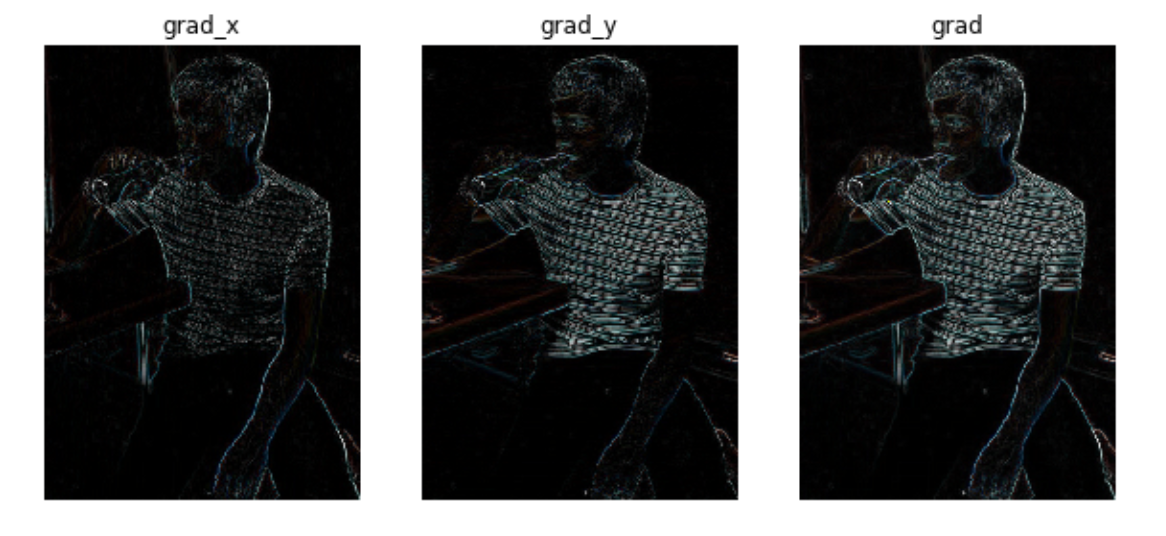
\includegraphics[width=0.9\textwidth]{gradients.png}
  \caption{左:横向梯度绝对值;中:纵向梯度绝对值;右:梯度大小}
  \label{fig:gradients}
\end{figure}

  图\ref{fig:gradients}中包括了RGB三个通道在每一个像素点上的梯度值,在计算HOG特征向量时,我们选取三个通道的梯度的最大值作为该点处的梯度大小,最大值对应的通道的梯度角度为该点处的梯度方向。

  方向梯度直方图统计的实际上是梯度的方向。梯度的方向在$[0^{\circ},360^{\circ})$上,但是我们实际在统计方向时,采用的却是$[0^{\circ},180^{\circ})$的统计范围,计算$\theta(x,y) mod 180^{\circ}$来代替原有的角度值,即将相差$180^{\circ}$的两个角度视为同一个梯度方向。已有实验表明,这种统计方式得到的结果往往比采用$[0^{\circ},360^{\circ})$范围的原方向更好。在统计梯度方向时时,我们还需要使用梯度的大小作为对应方向的权重。

  在计算直方图时,我们取9个组(bins),分别对应$0^{\circ},20^{\circ},40^{\circ},\dots,160^{\circ}$,若一个像素处的梯度正好为20的整数倍,将其梯度大小加到对应的bin中;否则,按照比例,将其加入相邻的两个bins中。以图\ref{fig:distribute}为例。

\begin{figure}[htb]
  \centering
  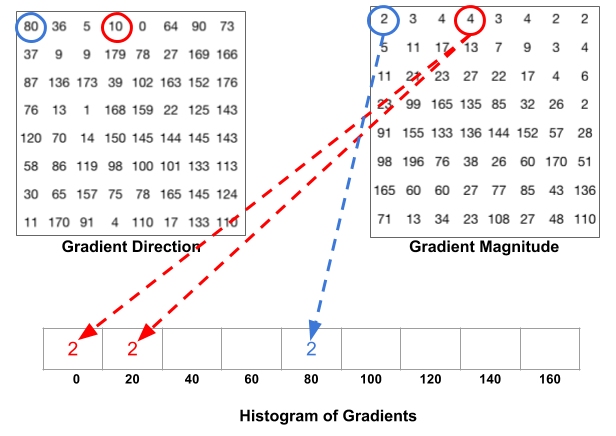
\includegraphics[width=0.8\textwidth]{calc_histogram.png}
  \caption{统计梯度方向直方图的方法示意}
  \label{fig:distribute}
\end{figure}

  

\paragraph{行人检测算法}

\subsubsection{深度学习}

\subsection{基于动态的追踪}


\section{激光行人追踪}


